%%%%%%%%%%%%%%%%%%%%%%%%%%%%%%%%%%%%%%%%%
% The Legrand Orange Book
% LaTeX Template
% Version 2.4 (26/09/2018)
%
% This template was downloaded from:
% http://www.LaTeXTemplates.com
%
% Original author:
% Mathias Legrand (legrand.mathias@gmail.com) with modifications by:
% Vel (vel@latextemplates.com)
%
% License:
% CC BY-NC-SA 3.0 (http://creativecommons.org/licenses/by-nc-sa/3.0/)
%
% Compiling this template:
% This template uses biber for its bibliography and makeindex for its index.
% When you first open the template, compile it from the command line with the 
% commands below to make sure your LaTeX distribution is configured correctly:
%
% 1) pdflatex main
% 2) makeindex main.idx -s StyleInd.ist
% 3) biber main
% 4) pdflatex main x 2
%
% After this, when you wish to update the bibliography/index use the appropriate
% command above and make sure to compile with pdflatex several times 
% afterwards to propagate your changes to the document.
%
% This template also uses a number of packages which may need to be
% updated to the newest versions for the template to compile. It is strongly
% recommended you update your LaTeX distribution if you have any
% compilation errors.
%
% Important note:
% Chapter heading images should have a 2:1 width:height ratio,
% e.g. 920px width and 460px height.
%
%%%%%%%%%%%%%%%%%%%%%%%%%%%%%%%%%%%%%%%%%

%----------------------------------------------------------------------------------------
%	PACKAGES AND OTHER DOCUMENT CONFIGURATIONS
%----------------------------------------------------------------------------------------

\documentclass[11pt,fleqn]{book} % Default font size and left-justified equations

%%%%%%%%%%%%%%%%%%%%%%%%%%%%%%%%%%%%%%%%%
% The Legrand Orange Book
% Structural Definitions File
% Version 2.1 (26/09/2018)
%
% Original author:
% Mathias Legrand (legrand.mathias@gmail.com) with modifications by:
% Vel (vel@latextemplates.com)
% 
% This file was downloaded from:
% http://www.LaTeXTemplates.com
%
% License:
% CC BY-NC-SA 3.0 (http://creativecommons.org/licenses/by-nc-sa/3.0/)
%
%%%%%%%%%%%%%%%%%%%%%%%%%%%%%%%%%%%%%%%%%

%----------------------------------------------------------------------------------------
%	VARIOUS REQUIRED PACKAGES AND CONFIGURATIONS
%----------------------------------------------------------------------------------------

\usepackage{graphicx} % Required for including pictures
\graphicspath{{Pictures/}} % Specifies the directory where pictures are stored

\usepackage{lipsum} % Inserts dummy text

\usepackage{tikz} % Required for drawing custom shapes

\usepackage[english]{babel} % English language/hyphenation

\usepackage{enumitem} % Customize lists
\setlist{nolistsep} % Reduce spacing between bullet points and numbered lists

\usepackage{booktabs} % Required for nicer horizontal rules in tables

\usepackage{xcolor} % Required for specifying colors by name
\definecolor{ocre}{RGB}{243,102,25} % Define the orange color used for highlighting throughout the book

%----------------------------------------------------------------------------------------
%	MARGINS
%----------------------------------------------------------------------------------------

\usepackage{geometry} % Required for adjusting page dimensions and margins

\geometry{
	paper=a4paper, % Paper size, change to letterpaper for US letter size
	top=3cm, % Top margin
	bottom=3cm, % Bottom margin
	left=3cm, % Left margin
	right=3cm, % Right margin
	headheight=14pt, % Header height
	footskip=1.4cm, % Space from the bottom margin to the baseline of the footer
	headsep=10pt, % Space from the top margin to the baseline of the header
	%showframe, % Uncomment to show how the type block is set on the page
}

%----------------------------------------------------------------------------------------
%	FONTS
%----------------------------------------------------------------------------------------

\usepackage{avant} % Use the Avantgarde font for headings
%\usepackage{times} % Use the Times font for headings
\usepackage{mathptmx} % Use the Adobe Times Roman as the default text font together with math symbols from the Sym­bol, Chancery and Com­puter Modern fonts

\usepackage{microtype} % Slightly tweak font spacing for aesthetics
\usepackage[utf8]{inputenc} % Required for including letters with accents
\usepackage[T1]{fontenc} % Use 8-bit encoding that has 256 glyphs

%----------------------------------------------------------------------------------------
%	BIBLIOGRAPHY AND INDEX
%----------------------------------------------------------------------------------------

\usepackage[style=numeric,citestyle=numeric,sorting=nyt,sortcites=true,autopunct=true,babel=hyphen,hyperref=true,abbreviate=false,backref=true,backend=biber]{biblatex}
\addbibresource{bibliography.bib} % BibTeX bibliography file
\defbibheading{bibempty}{}

\usepackage{calc} % For simpler calculation - used for spacing the index letter headings correctly
\usepackage{makeidx} % Required to make an index
\makeindex % Tells LaTeX to create the files required for indexing

%----------------------------------------------------------------------------------------
%	MAIN TABLE OF CONTENTS
%----------------------------------------------------------------------------------------

\usepackage{titletoc} % Required for manipulating the table of contents

\contentsmargin{0cm} % Removes the default margin

% Part text styling (this is mostly taken care of in the PART HEADINGS section of this file)
\titlecontents{part}
	[0cm] % Left indentation
	{\addvspace{20pt}\bfseries} % Spacing and font options for parts
	{}
	{}
	{}

% Chapter text styling
\titlecontents{chapter}
	[1.25cm] % Left indentation
	{\addvspace{12pt}\large\sffamily\bfseries} % Spacing and font options for chapters
	{\color{ocre!60}\contentslabel[\Large\thecontentslabel]{1.25cm}\color{ocre}} % Formatting of numbered sections of this type
	{\color{ocre}} % Formatting of numberless sections of this type
	{\color{ocre!60}\normalsize\;\titlerule*[.5pc]{.}\;\thecontentspage} % Formatting of the filler to the right of the heading and the page number

% Section text styling
\titlecontents{section}
	[1.25cm] % Left indentation
	{\addvspace{3pt}\sffamily\bfseries} % Spacing and font options for sections
	{\contentslabel[\thecontentslabel]{1.25cm}} % Formatting of numbered sections of this type
	{} % Formatting of numberless sections of this type
	{\hfill\color{black}\thecontentspage} % Formatting of the filler to the right of the heading and the page number

% Subsection text styling
\titlecontents{subsection}
	[1.25cm] % Left indentation
	{\addvspace{1pt}\sffamily\small} % Spacing and font options for subsections
	{\contentslabel[\thecontentslabel]{1.25cm}} % Formatting of numbered sections of this type
	{} % Formatting of numberless sections of this type
	{\ \titlerule*[.5pc]{.}\;\thecontentspage} % Formatting of the filler to the right of the heading and the page number

% Figure text styling
\titlecontents{figure}
	[1.25cm] % Left indentation
	{\addvspace{1pt}\sffamily\small} % Spacing and font options for figures
	{\thecontentslabel\hspace*{1em}} % Formatting of numbered sections of this type
	{} % Formatting of numberless sections of this type
	{\ \titlerule*[.5pc]{.}\;\thecontentspage} % Formatting of the filler to the right of the heading and the page number

% Table text styling
\titlecontents{table}
	[1.25cm] % Left indentation
	{\addvspace{1pt}\sffamily\small} % Spacing and font options for tables
	{\thecontentslabel\hspace*{1em}} % Formatting of numbered sections of this type
	{} % Formatting of numberless sections of this type
	{\ \titlerule*[.5pc]{.}\;\thecontentspage} % Formatting of the filler to the right of the heading and the page number

%----------------------------------------------------------------------------------------
%	MINI TABLE OF CONTENTS IN PART HEADS
%----------------------------------------------------------------------------------------

% Chapter text styling
\titlecontents{lchapter}
	[0em] % Left indentation
	{\addvspace{15pt}\large\sffamily\bfseries} % Spacing and font options for chapters
	{\color{ocre}\contentslabel[\Large\thecontentslabel]{1.25cm}\color{ocre}} % Chapter number
	{}  
	{\color{ocre}\normalsize\sffamily\bfseries\;\titlerule*[.5pc]{.}\;\thecontentspage} % Page number

% Section text styling
\titlecontents{lsection}
	[0em] % Left indentation
	{\sffamily\small} % Spacing and font options for sections
	{\contentslabel[\thecontentslabel]{1.25cm}} % Section number
	{}
	{}

% Subsection text styling (note these aren't shown by default, display them by searchings this file for tocdepth and reading the commented text)
\titlecontents{lsubsection}
	[.5em] % Left indentation
	{\sffamily\footnotesize} % Spacing and font options for subsections
	{\contentslabel[\thecontentslabel]{1.25cm}}
	{}
	{}

%----------------------------------------------------------------------------------------
%	HEADERS AND FOOTERS
%----------------------------------------------------------------------------------------

\usepackage{fancyhdr} % Required for header and footer configuration

\pagestyle{fancy} % Enable the custom headers and footers

\renewcommand{\chaptermark}[1]{\markboth{\sffamily\normalsize\bfseries\chaptername\ \thechapter.\ #1}{}} % Styling for the current chapter in the header
\renewcommand{\sectionmark}[1]{\markright{\sffamily\normalsize\thesection\hspace{5pt}#1}{}} % Styling for the current section in the header

\fancyhf{} % Clear default headers and footers
\fancyhead[LE,RO]{\sffamily\normalsize\thepage} % Styling for the page number in the header
\fancyhead[LO]{\rightmark} % Print the nearest section name on the left side of odd pages
\fancyhead[RE]{\leftmark} % Print the current chapter name on the right side of even pages
%\fancyfoot[C]{\thepage} % Uncomment to include a footer

\renewcommand{\headrulewidth}{0.5pt} % Thickness of the rule under the header

\fancypagestyle{plain}{% Style for when a plain pagestyle is specified
	\fancyhead{}\renewcommand{\headrulewidth}{0pt}%
}

% Removes the header from odd empty pages at the end of chapters
\makeatletter
\renewcommand{\cleardoublepage}{
\clearpage\ifodd\c@page\else
\hbox{}
\vspace*{\fill}
\thispagestyle{empty}
\newpage
\fi}

%----------------------------------------------------------------------------------------
%	THEOREM STYLES
%----------------------------------------------------------------------------------------

\usepackage{amsmath,amsfonts,amssymb,amsthm} % For math equations, theorems, symbols, etc

\newcommand{\intoo}[2]{\mathopen{]}#1\,;#2\mathclose{[}}
\newcommand{\ud}{\mathop{\mathrm{{}d}}\mathopen{}}
\newcommand{\intff}[2]{\mathopen{[}#1\,;#2\mathclose{]}}
\renewcommand{\qedsymbol}{$\blacksquare$}
\newtheorem{notation}{Notation}[chapter]

% Boxed/framed environments
\newtheoremstyle{ocrenumbox}% Theorem style name
{0pt}% Space above
{0pt}% Space below
{\normalfont}% Body font
{}% Indent amount
{\small\bf\sffamily\color{ocre}}% Theorem head font
{\;}% Punctuation after theorem head
{0.25em}% Space after theorem head
{\small\sffamily\color{ocre}\thmname{#1}\nobreakspace\thmnumber{\@ifnotempty{#1}{}\@upn{#2}}% Theorem text (e.g. Theorem 2.1)
\thmnote{\nobreakspace\the\thm@notefont\sffamily\bfseries\color{black}---\nobreakspace#3.}} % Optional theorem note

\newtheoremstyle{blacknumex}% Theorem style name
{5pt}% Space above
{5pt}% Space below
{\normalfont}% Body font
{} % Indent amount
{\small\bf\sffamily}% Theorem head font
{\;}% Punctuation after theorem head
{0.25em}% Space after theorem head
{\small\sffamily{\tiny\ensuremath{\blacksquare}}\nobreakspace\thmname{#1}\nobreakspace\thmnumber{\@ifnotempty{#1}{}\@upn{#2}}% Theorem text (e.g. Theorem 2.1)
\thmnote{\nobreakspace\the\thm@notefont\sffamily\bfseries---\nobreakspace#3.}}% Optional theorem note

\newtheoremstyle{blacknumbox} % Theorem style name
{0pt}% Space above
{0pt}% Space below
{\normalfont}% Body font
{}% Indent amount
{\small\bf\sffamily}% Theorem head font
{\;}% Punctuation after theorem head
{0.25em}% Space after theorem head
{\small\sffamily\thmname{#1}\nobreakspace\thmnumber{\@ifnotempty{#1}{}\@upn{#2}}% Theorem text (e.g. Theorem 2.1)
\thmnote{\nobreakspace\the\thm@notefont\sffamily\bfseries---\nobreakspace#3.}}% Optional theorem note

% Non-boxed/non-framed environments
\newtheoremstyle{ocrenum}% Theorem style name
{5pt}% Space above
{5pt}% Space below
{\normalfont}% Body font
{}% Indent amount
{\small\bf\sffamily\color{ocre}}% Theorem head font
{\;}% Punctuation after theorem head
{0.25em}% Space after theorem head
{\small\sffamily\color{ocre}\thmname{#1}\nobreakspace\thmnumber{\@ifnotempty{#1}{}\@upn{#2}}% Theorem text (e.g. Theorem 2.1)
\thmnote{\nobreakspace\the\thm@notefont\sffamily\bfseries\color{black}---\nobreakspace#3.}} % Optional theorem note
\makeatother

% Defines the theorem text style for each type of theorem to one of the three styles above
\newcounter{dummy} 
\numberwithin{dummy}{section}
\theoremstyle{ocrenumbox}
\newtheorem{theoremeT}[dummy]{Theorem}
\newtheorem{toolboxT}[dummy]{Toolbox}
\newtheorem{problem}{Problem}[chapter]
\newtheorem{exerciseT}{Exercise}[chapter]
\theoremstyle{blacknumex}
\newtheorem{exampleT}{Example}[chapter]
\theoremstyle{blacknumbox}
\newtheorem{vocabulary}{Vocabulary}[chapter]
\newtheorem{definitionT}{Definition}[section]
\newtheorem{corollaryT}[dummy]{Corollary}
\theoremstyle{ocrenum}
\newtheorem{proposition}[dummy]{Proposition}

%----------------------------------------------------------------------------------------
%	DEFINITION OF COLORED BOXES
%----------------------------------------------------------------------------------------

\RequirePackage[framemethod=default]{mdframed} % Required for creating the theorem, definition, exercise and corollary boxes

% Theorem box
\newmdenv[skipabove=7pt,
skipbelow=7pt,
backgroundcolor=black!5,
linecolor=ocre,
innerleftmargin=5pt,
innerrightmargin=5pt,
innertopmargin=5pt,
leftmargin=0cm,
rightmargin=0cm,
innerbottommargin=5pt]{tBox}

% Exercise box	  
\newmdenv[skipabove=7pt,
skipbelow=7pt,
rightline=false,
leftline=true,
topline=false,
bottomline=false,
backgroundcolor=ocre!10,
linecolor=ocre,
innerleftmargin=5pt,
innerrightmargin=5pt,
innertopmargin=5pt,
innerbottommargin=5pt,
leftmargin=0cm,
rightmargin=0cm,
linewidth=4pt]{eBox}	

% Definition box
\newmdenv[skipabove=7pt,
skipbelow=7pt,
rightline=false,
leftline=true,
topline=false,
bottomline=false,
linecolor=ocre,
innerleftmargin=5pt,
innerrightmargin=5pt,
innertopmargin=0pt,
leftmargin=0cm,
rightmargin=0cm,
linewidth=4pt,
innerbottommargin=0pt]{dBox}	

% Corollary box
\newmdenv[skipabove=7pt,
skipbelow=7pt,
rightline=false,
leftline=true,
topline=false,
bottomline=false,
linecolor=gray,
backgroundcolor=black!5,
innerleftmargin=5pt,
innerrightmargin=5pt,
innertopmargin=5pt,
leftmargin=0cm,
rightmargin=0cm,
linewidth=4pt,
innerbottommargin=5pt]{cBox}

% Creates an environment for each type of theorem and assigns it a theorem text style from the "Theorem Styles" section above and a colored box from above
\newenvironment{theorem}{\begin{tBox}\begin{theoremeT}}{\end{theoremeT}\end{tBox}}
\newenvironment{toolbox}{\begin{tBox}\begin{toolboxT}}{\end{toolboxT}\end{tBox}}
\newenvironment{exercise}{\begin{eBox}\begin{exerciseT}}{\hfill{\color{ocre}\tiny\ensuremath{\blacksquare}}\end{exerciseT}\end{eBox}}				  
\newenvironment{definition}{\begin{dBox}\begin{definitionT}}{\end{definitionT}\end{dBox}}	
\newenvironment{example}{\begin{exampleT}}{\hfill{\tiny\ensuremath{\blacksquare}}\end{exampleT}}		
\newenvironment{corollary}{\begin{cBox}\begin{corollaryT}}{\end{corollaryT}\end{cBox}}	

%----------------------------------------------------------------------------------------
%	REMARK ENVIRONMENT
%----------------------------------------------------------------------------------------

\newenvironment{remark}{\par\vspace{10pt}\small % Vertical white space above the remark and smaller font size
\begin{list}{}{
\leftmargin=35pt % Indentation on the left
\rightmargin=25pt}\item\ignorespaces % Indentation on the right
\makebox[-2.5pt]{\begin{tikzpicture}[overlay]
\node[draw=ocre!60,line width=1pt,circle,fill=ocre!25,font=\sffamily\bfseries,inner sep=2pt,outer sep=0pt] at (-15pt,0pt){\textcolor{ocre}{R}};\end{tikzpicture}} % Orange R in a circle
\advance\baselineskip -1pt}{\end{list}\vskip5pt} % Tighter line spacing and white space after remark

%----------------------------------------------------------------------------------------
%	SECTION NUMBERING IN THE MARGIN
%----------------------------------------------------------------------------------------

\makeatletter
\renewcommand{\@seccntformat}[1]{\llap{\textcolor{ocre}{\csname the#1\endcsname}\hspace{1em}}}                    
\renewcommand{\section}{\@startsection{section}{1}{\z@}
{-4ex \@plus -1ex \@minus -.4ex}
{1ex \@plus.2ex }
{\normalfont\large\sffamily\bfseries}}
\renewcommand{\subsection}{\@startsection {subsection}{2}{\z@}
{-3ex \@plus -0.1ex \@minus -.4ex}
{0.5ex \@plus.2ex }
{\normalfont\sffamily\bfseries}}
\renewcommand{\subsubsection}{\@startsection {subsubsection}{3}{\z@}
{-2ex \@plus -0.1ex \@minus -.2ex}
{.2ex \@plus.2ex }
{\normalfont\small\sffamily\bfseries}}                        
\renewcommand\paragraph{\@startsection{paragraph}{4}{\z@}
{-2ex \@plus-.2ex \@minus .2ex}
{.1ex}
{\normalfont\small\sffamily\bfseries}}

%----------------------------------------------------------------------------------------
%	PART HEADINGS
%----------------------------------------------------------------------------------------

% Numbered part in the table of contents
\newcommand{\@mypartnumtocformat}[2]{%
	\setlength\fboxsep{0pt}%
	\noindent\colorbox{ocre!20}{\strut\parbox[c][.7cm]{\ecart}{\color{ocre!70}\Large\sffamily\bfseries\centering#1}}\hskip\esp\colorbox{ocre!40}{\strut\parbox[c][.7cm]{\linewidth-\ecart-\esp}{\Large\sffamily\centering#2}}%
}

% Unnumbered part in the table of contents
\newcommand{\@myparttocformat}[1]{%
	\setlength\fboxsep{0pt}%
	\noindent\colorbox{ocre!40}{\strut\parbox[c][.7cm]{\linewidth}{\Large\sffamily\centering#1}}%
}

\newlength\esp
\setlength\esp{4pt}
\newlength\ecart
\setlength\ecart{1.2cm-\esp}
\newcommand{\thepartimage}{}%
\newcommand{\partimage}[1]{\renewcommand{\thepartimage}{#1}}%
\def\@part[#1]#2{%
\ifnum \c@secnumdepth >-2\relax%
\refstepcounter{part}%
\addcontentsline{toc}{part}{\texorpdfstring{\protect\@mypartnumtocformat{\thepart}{#1}}{\partname~\thepart\ ---\ #1}}
\else%
\addcontentsline{toc}{part}{\texorpdfstring{\protect\@myparttocformat{#1}}{#1}}%
\fi%
\startcontents%
\markboth{}{}%
{\thispagestyle{empty}%
\begin{tikzpicture}[remember picture,overlay]%
\node at (current page.north west){\begin{tikzpicture}[remember picture,overlay]%	
\fill[ocre!20](0cm,0cm) rectangle (\paperwidth,-\paperheight);
\node[anchor=north] at (4cm,-3.25cm){\color{ocre!40}\fontsize{220}{100}\sffamily\bfseries\thepart}; 
\node[anchor=south east] at (\paperwidth-1cm,-\paperheight+1cm){\parbox[t][][t]{8.5cm}{
\printcontents{l}{0}{\setcounter{tocdepth}{1}}% The depth to which the Part mini table of contents displays headings; 0 for chapters only, 1 for chapters and sections and 2 for chapters, sections and subsections
}};
\node[anchor=north east] at (\paperwidth-1.5cm,-3.25cm){\parbox[t][][t]{15cm}{\strut\raggedleft\color{white}\fontsize{30}{30}\sffamily\bfseries#2}};
\end{tikzpicture}};
\end{tikzpicture}}%
\@endpart}
\def\@spart#1{%
\startcontents%
\phantomsection
{\thispagestyle{empty}%
\begin{tikzpicture}[remember picture,overlay]%
\node at (current page.north west){\begin{tikzpicture}[remember picture,overlay]%	
\fill[ocre!20](0cm,0cm) rectangle (\paperwidth,-\paperheight);
\node[anchor=north east] at (\paperwidth-1.5cm,-3.25cm){\parbox[t][][t]{15cm}{\strut\raggedleft\color{white}\fontsize{30}{30}\sffamily\bfseries#1}};
\end{tikzpicture}};
\end{tikzpicture}}
\addcontentsline{toc}{part}{\texorpdfstring{%
\setlength\fboxsep{0pt}%
\noindent\protect\colorbox{ocre!40}{\strut\protect\parbox[c][.7cm]{\linewidth}{\Large\sffamily\protect\centering #1\quad\mbox{}}}}{#1}}%
\@endpart}
\def\@endpart{\vfil\newpage
\if@twoside
\if@openright
\null
\thispagestyle{empty}%
\newpage
\fi
\fi
\if@tempswa
\twocolumn
\fi}

%----------------------------------------------------------------------------------------
%	CHAPTER HEADINGS
%----------------------------------------------------------------------------------------

% A switch to conditionally include a picture, implemented by Christian Hupfer
\newif\ifusechapterimage
\usechapterimagetrue
\newcommand{\thechapterimage}{}%
\newcommand{\chapterimage}[1]{\ifusechapterimage\renewcommand{\thechapterimage}{#1}\fi}%
\newcommand{\autodot}{.}
\def\@makechapterhead#1{%
{\parindent \z@ \raggedright \normalfont
\ifnum \c@secnumdepth >\m@ne
\if@mainmatter
\begin{tikzpicture}[remember picture,overlay]
\node at (current page.north west)
{\begin{tikzpicture}[remember picture,overlay]
\node[anchor=north west,inner sep=0pt] at (0,0) {\ifusechapterimage\includegraphics[width=\paperwidth]{\thechapterimage}\fi};
\draw[anchor=west] (\Gm@lmargin,-9cm) node [line width=2pt,rounded corners=15pt,draw=ocre,fill=white,fill opacity=0.5,inner sep=15pt]{\strut\makebox[22cm]{}};
\draw[anchor=west] (\Gm@lmargin+.3cm,-9cm) node {\huge\sffamily\bfseries\color{black}\thechapter\autodot~#1\strut};
\end{tikzpicture}};
\end{tikzpicture}
\else
\begin{tikzpicture}[remember picture,overlay]
\node at (current page.north west)
{\begin{tikzpicture}[remember picture,overlay]
\node[anchor=north west,inner sep=0pt] at (0,0) {\ifusechapterimage\includegraphics[width=\paperwidth]{\thechapterimage}\fi};
\draw[anchor=west] (\Gm@lmargin,-9cm) node [line width=2pt,rounded corners=15pt,draw=ocre,fill=white,fill opacity=0.5,inner sep=15pt]{\strut\makebox[22cm]{}};
\draw[anchor=west] (\Gm@lmargin+.3cm,-9cm) node {\huge\sffamily\bfseries\color{black}#1\strut};
\end{tikzpicture}};
\end{tikzpicture}
\fi\fi\par\vspace*{270\p@}}}

%-------------------------------------------

\def\@makeschapterhead#1{%
\begin{tikzpicture}[remember picture,overlay]
\node at (current page.north west)
{\begin{tikzpicture}[remember picture,overlay]
\node[anchor=north west,inner sep=0pt] at (0,0) {\ifusechapterimage\includegraphics[width=\paperwidth]{\thechapterimage}\fi};
\draw[anchor=west] (\Gm@lmargin,-9cm) node [line width=2pt,rounded corners=15pt,draw=ocre,fill=white,fill opacity=0.5,inner sep=15pt]{\strut\makebox[22cm]{}};
\draw[anchor=west] (\Gm@lmargin+.3cm,-9cm) node {\huge\sffamily\bfseries\color{black}#1\strut};
\end{tikzpicture}};
\end{tikzpicture}
\par\vspace*{270\p@}}
\makeatother

%----------------------------------------------------------------------------------------
%	LINKS
%----------------------------------------------------------------------------------------

\usepackage{hyperref}
\hypersetup{hidelinks,backref=true,pagebackref=true,hyperindex=true,colorlinks=false,breaklinks=true,urlcolor=ocre,bookmarks=true,bookmarksopen=false}

\usepackage{bookmark}
\bookmarksetup{
open,
numbered,
addtohook={%
\ifnum\bookmarkget{level}=0 % chapter
\bookmarksetup{bold}%
\fi
\ifnum\bookmarkget{level}=-1 % part
\bookmarksetup{color=ocre,bold}%
\fi
}
}

%----------------------------------------------------------------------------------------
%	CODE
%----------------------------------------------------------------------------------------

%Needs xcolor
\usepackage{minted}
\definecolor{LightGray}{gray}{0.95}

\newcommand{\BatFancyFormatLine}{%
  \def\FancyVerbFormatLine##1{> \,##1}%
}

\newcommand{\PythonFancyFormatLine}{%
  \def\FancyVerbFormatLine##1{{>}{>}{>} \,##1}%
}

\newenvironment{script}
{\VerbatimEnvironment\begin{minted}[mathescape,
               linenos,
               numbersep=5pt,
               gobble=0,
               bgcolor=LightGray,
               frame=lines,
               framesep=2mm]{python}}
{\end{minted}}

\newenvironment{cmd}
{\VerbatimEnvironment\begin{minted}[formatcom=\BatFancyFormatLine ,
               frame=lines,
               framesep=2mm]{bat}}
{\end{minted}}

\newenvironment{shell}
{\VerbatimEnvironment\begin{minted}[formatcom=\PythonFancyFormatLine ,
               numbersep=5pt,
               gobble=0,
               bgcolor=LightGray,
               frame=lines,
               framesep=2mm]{python}}
{\end{minted}}

%Inline code
\newcommand{\icd}[1]{\textbf{#1}}

%----------------------------------------------------------------------------------------
%	TEXT FORMATTING
%----------------------------------------------------------------------------------------

%----------------------------------------------------------------------------------------
%	Summary Box
%----------------------------------------------------------------------------------------
  
\definecolor{LightBlue}{RGB}{0,0,50}

\newmdenv[skipabove=7pt,
skipbelow=7pt,
rightline=false,
leftline=true,
topline=false,
bottomline=false,
backgroundcolor=LightBlue!10,
linecolor=LightBlue,
innerleftmargin=5pt,
innerrightmargin=5pt,
innertopmargin=5pt,
innerbottommargin=5pt,
leftmargin=0cm,
rightmargin=0cm,
linewidth=4pt]{summaryBox}	 % Insert the commands.tex file which contains the majority of the structure behind the template

%\hypersetup{pdftitle={Title},pdfauthor={Author}} % Uncomment and fill out to include PDF metadata for the author and title of the book

%----------------------------------------------------------------------------------------

\begin{document}

%----------------------------------------------------------------------------------------
%	TITLE PAGE
%----------------------------------------------------------------------------------------

\begingroup
\thispagestyle{empty} % Suppress headers and footers on the title page
\begin{tikzpicture}[remember picture,overlay]
\node[inner sep=0pt] (background) at (current page.center) {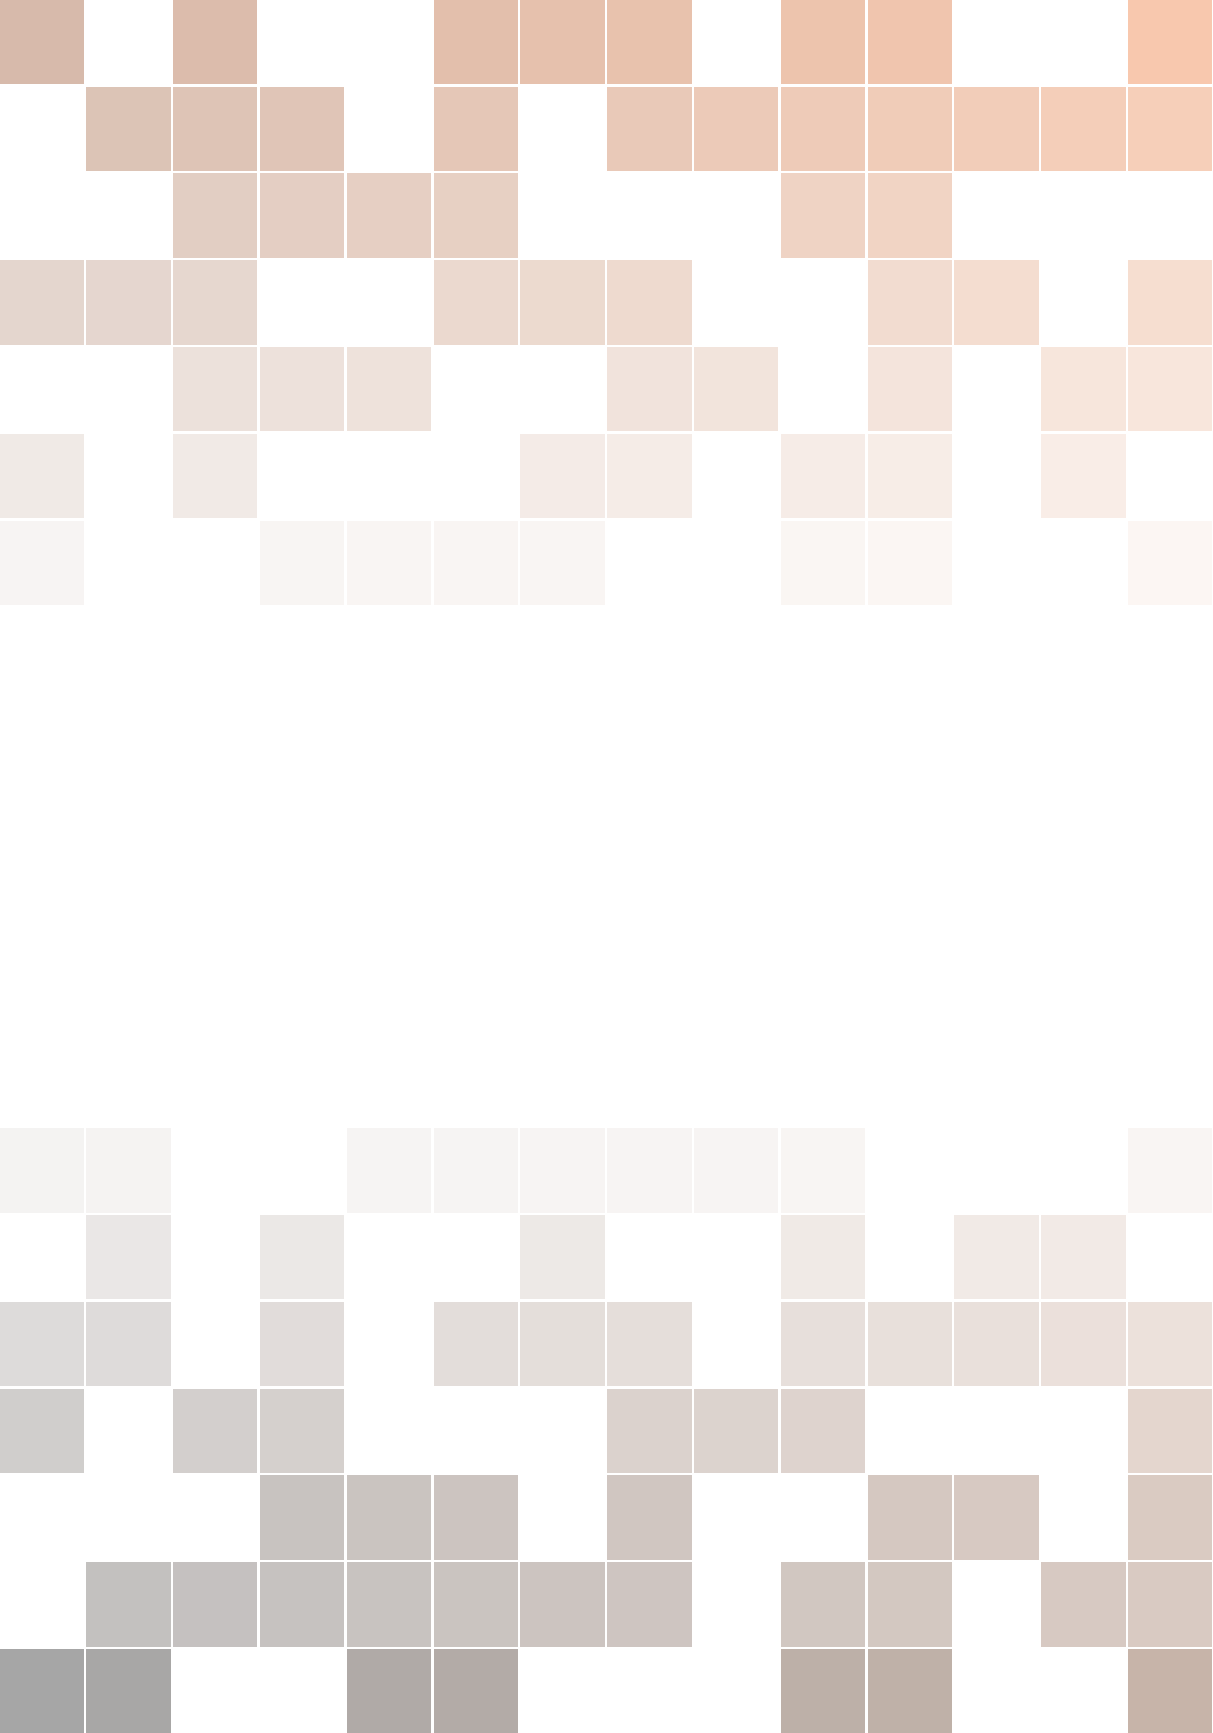
\includegraphics[width=\paperwidth]{background.pdf}};
\draw (current page.center) node [fill=ocre!30!white,fill opacity=0.6,text opacity=1,inner sep=1cm]{\Huge\centering\bfseries\sffamily\parbox[c][][t]{\paperwidth}{\centering The Search for a Title\\[15pt] % Book title
{\Large A Profound Subtitle}\\[20pt] % Subtitle
{\huge Author}}}; % Author name
\end{tikzpicture}
\vfill
\endgroup

%----------------------------------------------------------------------------------------
%	COPYRIGHT PAGE
%----------------------------------------------------------------------------------------

\newpage
~\vfill
\thispagestyle{empty}

\noindent Copyright \copyright\ 2019 John Smith\\ % Copyright notice

\noindent \textsc{Published by Publisher}\\ % Publisher

\noindent \textsc{www.zimcode.org}\\ % URL

\noindent Licensed under the Creative Commons Attribution-NonCommercial 3.0 Unported License (the ``License''). You may not use this file except in compliance with the License. You may obtain a copy of the License at \url{http://creativecommons.org/licenses/by-nc/3.0}. Unless required by applicable law or agreed to in writing, software distributed under the License is distributed on an \textsc{``as is'' basis, without warranties or conditions of any kind}, either express or implied. See the License for the specific language governing permissions and limitations under the License.\\ % License information, replace this with your own license (if any)

\noindent \textit{First printing, March 2019} % Printing/edition date

%----------------------------------------------------------------------------------------
%	TABLE OF CONTENTS
%----------------------------------------------------------------------------------------

%\usechapterimagefalse % If you don't want to include a chapter image, use this to toggle images off - it can be enabled later with \usechapterimagetrue

\chapterimage{chapter_head_1.pdf} % Table of contents heading image

\pagestyle{empty} % Disable headers and footers for the following pages

\tableofcontents % Print the table of contents itself

\cleardoublepage % Forces the first chapter to start on an odd page so it's on the right side of the book

\pagestyle{fancy} % Enable headers and footers again

%----------------------------------------------------------------------------------------
%	PART
%----------------------------------------------------------------------------------------

\part{Part One}

%----------------------------------------------------------------------------------------
%	CHAPTERS
%----------------------------------------------------------------------------------------

\chapterimage{chapter_head_2.pdf} % Chapter heading image

\chapter{Introduction to Computers and Programming}

\section{Paragraphs of Text}\index{Paragraphs of Text}
Blah blah blah

%------------------------------------------------

\section{Citation}\index{Citation}

This statement requires citation \cite{article_key}; this one is more specific \cite[162]{book_key}.

%------------------------------------------------

\section{Lists}\index{Lists}

Lists are useful to present information in a concise and/or ordered way\footnote{Footnote example...}.

\subsection{Numbered List}\index{Lists!Numbered List}

\begin{enumerate}
\item The first item
\item The second item
\item The third item
\end{enumerate}

\subsection{Bullet Points}\index{Lists!Bullet Points}

\begin{itemize}
\item The first item
\item The second item
\item The third item
\end{itemize}

\subsection{Descriptions and Definitions}\index{Lists!Descriptions and Definitions}

\begin{description}
\item[Name] Description
\item[Word] Definition
\item[Comment] Elaboration
\end{description}

\section{Theorems}\index{Theorems}

This is an example of theorems.

\subsection{Several equations}\index{Theorems!Several Equations}
This is a theorem consisting of several equations.

\begin{theorem}[Name of the theorem]
In $E=\mathbb{R}^n$ all norms are equivalent. It has the properties:
\begin{align}
& \big| ||\mathbf{x}|| - ||\mathbf{y}|| \big|\leq || \mathbf{x}- \mathbf{y}||\\
&  ||\sum_{i=1}^n\mathbf{x}_i||\leq \sum_{i=1}^n||\mathbf{x}_i||\quad\text{where $n$ is a finite integer}
\end{align}
\end{theorem}

\subsection{Single Line}\index{Theorems!Single Line}
This is a theorem consisting of just one line.

\begin{theorem}
A set $\mathcal{D}(G)$ in dense in $L^2(G)$, $|\cdot|_0$. 
\end{theorem}

%------------------------------------------------

\section{Definitions}\index{Definitions}

This is an example of a definition. A definition could be mathematical or it could define a concept.

\begin{definition}[Definition name]
Given a vector space $E$, a norm on $E$ is an application, denoted $||\cdot||$, $E$ in $\mathbb{R}^+=[0,+\infty[$ such that:
\begin{align}
& ||\mathbf{x}||=0\ \Rightarrow\ \mathbf{x}=\mathbf{0}\\
& ||\lambda \mathbf{x}||=|\lambda|\cdot ||\mathbf{x}||\\
& ||\mathbf{x}+\mathbf{y}||\leq ||\mathbf{x}||+||\mathbf{y}||
\end{align}
\end{definition}

%------------------------------------------------

\section{Notations}\index{Notations}

\begin{notation}
Given an open subset $G$ of $\mathbb{R}^n$, the set of functions $\varphi$ are:
\begin{enumerate}
\item Bounded support $G$;
\item Infinitely differentiable;
\end{enumerate}
a vector space is denoted by $\mathcal{D}(G)$. 
\end{notation}

%------------------------------------------------

\section{Remarks}\index{Remarks}

This is an example of a remark.

\begin{remark}
The concepts presented here are now in conventional employment in mathematics. Vector spaces are taken over the field $\mathbb{K}=\mathbb{R}$, however, established properties are easily extended to $\mathbb{K}=\mathbb{C}$.
\end{remark}

%------------------------------------------------

\section{Corollaries}\index{Corollaries}

This is an example of a corollary.

\begin{corollary}[Corollary name]
The concepts presented here are now in conventional employment in mathematics. Vector spaces are taken over the field $\mathbb{K}=\mathbb{R}$, however, established properties are easily extended to $\mathbb{K}=\mathbb{C}$.
\end{corollary}

%------------------------------------------------

\section{Propositions}\index{Propositions}

This is an example of propositions.

\subsection{Several equations}\index{Propositions!Several Equations}

\begin{proposition}[Proposition name]
It has the properties:
\begin{align}
& \big| ||\mathbf{x}|| - ||\mathbf{y}|| \big|\leq || \mathbf{x}- \mathbf{y}||\\
&  ||\sum_{i=1}^n\mathbf{x}_i||\leq \sum_{i=1}^n||\mathbf{x}_i||\quad\text{where $n$ is a finite integer}
\end{align}
\end{proposition}

\subsection{Single Line}\index{Propositions!Single Line}

\begin{proposition} 
Let $f,g\in L^2(G)$; if $\forall \varphi\in\mathcal{D}(G)$, $(f,\varphi)_0=(g,\varphi)_0$ then $f = g$. 
\end{proposition}

%------------------------------------------------

\section{Examples}\index{Examples}

This is an example of examples.

\subsection{Equation and Text}\index{Examples!Equation and Text}

\begin{example}
Let $G=\{x\in\mathbb{R}^2:|x|<3\}$ and denoted by: $x^0=(1,1)$; consider the function:
\begin{equation}
f(x)=\left\{\begin{aligned} & \mathrm{e}^{|x|} & & \text{si $|x-x^0|\leq 1/2$}\\
& 0 & & \text{si $|x-x^0|> 1/2$}\end{aligned}\right.
\end{equation}
The function $f$ has bounded support, we can take $A=\{x\in\mathbb{R}^2:|x-x^0|\leq 1/2+\epsilon\}$ for all $\epsilon\in\intoo{0}{5/2-\sqrt{2}}$.
\end{example}

\subsection{Paragraph of Text}\index{Examples!Paragraph of Text}

\begin{example}[Example name]
\lipsum[2]
\end{example}

%------------------------------------------------

\section{Exercises}\index{Exercises}

This is an example of an exercise.

\begin{exercise}
This is a good place to ask a question to test learning progress or further cement ideas into students' minds.
\end{exercise}

%------------------------------------------------

\section{Problems}\index{Problems}

\begin{problem}
What is the average airspeed velocity of an unladen swallow?
\end{problem}

%------------------------------------------------

\section{Vocabulary}\index{Vocabulary}

Define a word to improve a students' vocabulary.

\begin{vocabulary}[Word]
Definition of word.
\end{vocabulary}

\section{Figure}\index{Figure}

\begin{figure}[h]
\centering
\includegraphics[scale=0.5]{placeholder.jpg}
\caption{Figure caption}
\label{fig:placeholder} % Unique label used for referencing the figure in-text
%\addcontentsline{toc}{figure}{Figure \ref{fig:placeholder}} % Uncomment to add the figure to the table of contents
\end{figure}

Referencing Figure \ref{fig:placeholder} in-text automatically.

\section{Table}\index{Table}

\begin{table}[h]
\centering
\begin{tabular}{l l l}
\toprule
\textbf{Treatments} & \textbf{Response 1} & \textbf{Response 2}\\
\midrule
Treatment 1 & 0.0003262 & 0.562 \\
Treatment 2 & 0.0015681 & 0.910 \\
Treatment 3 & 0.0009271 & 0.296 \\
\bottomrule
\end{tabular}
\caption{Table caption}
\label{tab:example} % Unique label used for referencing the table in-text
%\addcontentsline{toc}{table}{Table \ref{tab:example}} % Uncomment to add the table to the table of contents
\end{table}

\section{Code}

If code is in a file you can use

\inputminted{python}{Introduction/code.py}

Note that the path must be relative to the main.tex directory\\
\newline
For one line code

\mint{html}|<h2>Something <b>here</b></h2>|

For a python script

\begin{script}
def f():
	return True
\end{script}

For a python shell

\begin{shell}
'1' in '4521'
\end{shell}

For a cmd prompt

\begin{cmd}
dir
cd
cd ..
\end{cmd}

\chapterimage{chapter_head_2.pdf} % Chapter heading image

\chapter{Introduction to Computers and Python}

\section{Introduction to Computers}

A computer is a programmable electronic device that manipulates information, or data. It has the ability to store, retrieve, and process data. Your laptop, desktop, smartphone or tablet are all examples of computers.

\noindent The computer system is made up of three things:
\begin{description}
\item[Input] – This is the information that a computer gets from outside, it will never act on its
own e.g. when you type or touch a screen or talk into a microphone, you are giving an input of character. Things like keyboards, mice and touchscreens are called input devices.\\
\item[Output] – This is what the computer gives out e.g. the picture on your screen, a sound or turning off the lights.\\
\item[Processing] – These are the instructions and calculations that the computer must follow to do something with the input. For all the devices you use, you are used to being 
involved with the input and output part. In programming, you get to directly design
the processing part of a computer.\\
\end{description}

\begin{problem}
Can you name different examples of input, processing, output devices?
\end{problem}

\begin{figure}[h]
\centering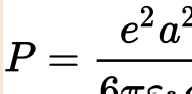
\includegraphics[width=\linewidth]{Chapter_One/Figures/a.png}
\caption{(Figure 1) Picture of the Computer Model: {a}}
\label{fig:model} % Unique label used for referencing the figure in-text
%\addcontentsline{toc}{figure}{Figure \ref{fig:placeholder}} % Uncomment to add the figure to the table of contents
\end{figure}

Here is how to think about the way a computer works that you should use about throughout this entire book. 
\begin{remark}
A computer takes inputs and processes them using a set of rules designed by a programmer(a human) to produce an output.
\end{remark}

The fact that the rules that govern a computer are designed by a human is very important. It means that computers can make mistakes if the human programmers made mistakes! The computer will follow instructions exactly as you \textit{program} it to, not exactly as you \textit{want} it to. As you start your journey as a programmer, you will make lots of mistakes and that is normal but it is important to remember to make sure things work properly, we will try and teach you how in this book.

\subsection{Operating Systems}

An operating system is the primary software that manages all the hardware  (screen, keyboard, touchscreen etc.) and software (Microsoft Word, Google Chrome, Whatsapp etc.) on a computer. The operating system, also known as an “OS,” \textit{interfaces} (connects) with the computer’s hardware and provides services that applications can use. For example, if you click print in Microsoft Word, Word sends the document you want to print to the OS, which in turn communicates with the printer using special software called "drivers" in order to tell the cartridge or laser inside the printer what shapes to make on the paper using ink.

Examples of Operating Systems are: Windows 10, MAC-OS, LINUX etc. Operating Systems are constantly being updated to work more efficiently and cater to new demands. This course uses Windows since that is the most popular OS available in Zimbabwe.
%
\begin{figure}[h]
\centering
\includegraphics[scale=0.5]{placeholder.jpg}
\caption{(Figure 2) Icons from various operating systems: {null - needs to be made}}
\label{fig:placeholder} % Unique label used for referencing the figure in-text
%\addcontentsline{toc}{figure}{Figure \ref{fig:placeholder}} % Uncomment to add the figure to the table of contents
\end{figure}
%

\subsection{File Systems}
One of the crucial things an OS does is to organize our files and folders: documents, movies, pictures, etc. A file system is a way of organizing and storing files on a hard drive, flash drive, or any other storage device.

\begin{definition}[Hard drive] A storage device for data. Data is any kind of information like pictures, documents, videos, music etc. All the data your computer needs to function will be stored there.
\end{definition}

In Windows, the Hard Drive on your computer is usually denoted as "C:" although it can be denoted by other letters. C: means all the stuff stored on this hard drive. In that C:, you can have files and folders inside it.

\begin{definition}[File] Anything that stores data that can be opened by a special program e.g. an mp3 file can be opened by a nusic player, a .docx file can be opened by Microsoft Word, An executable file can run by the OS, a .py file can be run by the Python interpretor.
\end{definition}

There are many different types of files, and their type is determined by their extensions. For example, you can tell that \textit{ZimCode.txt} is a text file because of it's extension \textit{.txt} at the end of the file name. This extension is important because it helps the OS know how to open and edit that file. If you click a .txt file, the OS will use Notepad or MS Word to open it. If you click a .mp3 file, the OS will use a Media Player to open it. It decides how to open the files using their extension.

\begin{definition}[Folder/Directory] The software object that stores files or other folders in a file system. It is also called a \textit{directory}. It is not a file, but just a storage location for files and folders. 
\end{definition}

Here is an example of a folder structure:

%
\begin{figure}[h]
\centering
\includegraphics[scale=0.5]{placeholder.jpg}
\caption{Image of a folder hierachy from windows explorer, preferably showing C:/, Users, Documents, Pictures etc. and matching the description below}
\label{fig:filehierachy} % Unique label used for referencing the figure in-text
%\addcontentsline{toc}{figure}{Figure \ref{fig:placeholder}} % Uncomment to add the figure to the table of contents
\end{figure}
%

Figure \ref{fig:filehierachy} shows a folder "hierachy" that shows you what is contained in each folder. Notice that the harddrive C: is at the root meaning that everything is stored on C:. The folder "Documents" is inside the folder ZimCode which is inside the folder Users and contains 3 files and 1 folder. The folder inside it contains 2 files. The folder doesn't have any extensions on it because it doesn't store any data on it's own. It is just a storage reference location for files and other folders.
Think of it as a paper bag. You can put an apple, banana and water bottle inside it. You can also put another paper bag inside the paper bag with pencils. And so on, and so forth.

\begin{definition}[Path] The location of a file or folder on the hard drive for a given filesystem. This is similar to the address of the place where you live. In computer terms, we commonly refer to it as a path i.e. the path you need to take to reach the folder/file. The path of "Star Wars: A New Hope (1977).mp4" could be something like "C:$\backslash$Users$\backslash$ZimCode$\backslash$Documents$\backslash$Star Wars: A New Hope (1977).mp4". Notice that the "Documents" folder is stored in another folder. Just like addresses, it is impossible for 2 files to have the same address on one computer. 
\end{definition}

\begin{problem}Can you think of why it would be bad for two files to have the same path?\end{problem}

\subsection{The Command Line and the Graphic User Interface (GUI)}

A GUI (graphical user interface) is a system of interactive visual components for computers. It helps us visualize the files stored on a computer in a human-readable format. For examples, if you want to open the Movies folder to watch your favorite action film stored inside, all you do is move the mouse cursor over the Movies folder and click on it. The whatsapp symbol is also an example of GUI component that you touch to open Whatsapp on a phone.

\begin{example}
Example where they create a new folder and open a file using the GUI
\end{example}

Before we had the GUI, we only had the Command Line Interface (CLI). Back then, if you wanted to watch your favorite film, you had to do so by typing a command in the command line. This is like what they do in the movies with hackers. 

To open the command line (a program called command prompt) in Windows, go to start and type \textbf{cmd} and press enter. You can open command prompt any other way you like. You should see a screen like the one shown in Figure \ref{fig:cmd}.

Generally, your command has to specify some or all of the following, using memorized keywords:

\begin{enumerate}
\item The name of the program you are using to perform the action.
\item The path of the file you want to perform an action on.
\item The specific action you want to perform.
\item Optional parameters of the action e.g. how many times you want to perform the action
\end{enumerate}

\begin{figure}[h]
\centering
\includegraphics[scale=0.5]{placeholder.jpg}
\caption{ Command line figure showing the same Documents folder as above}
\label{fig:cmd} 
\end{figure}

If all I had was the command line, instead of right-clicking my movie file, clicking Open with, and choosing VLC Media Player I would have to type a command like this in the command line to watch it:

\begin{cmd}
start vlc "C:\Users\ZimCode\Documents\Star Wars: A New Hope (1977).mp4".
\end{cmd}

Imagine having to do this every time you want do anything on a computer? Well, before the invention of the GUI, that is how people generally did things. An example of an early operating system that used this system is MS-DOS, which stands for Microsoft Disk Operating System

We still have the Command Line in modern computers because it helps us complete certain tasks quickly and more concisely. We can do most of the things we can do using a GUI with the CLI, in the following example, we repeat what we did before but this time using the CLI.

\begin{example}
Example where they create a new folder and open the same file using the command line
\end{example}

Here are some more basic command line commands:

\begin{itemize}
\item \textbf{help} - line lists all the basic built-in commands at your disposal.
\item \textbf{dir} - list all the contents inside the current directory
\item \textbf{cd} - change directory
\item \textbf{mkdir} - make a new directory
\item \textbf{cls} - clear the contents of the command line screen
\end{itemize}


\begin{exercise}\textbf{Master Hacker!}

You are going to use the following commands on the command line (Command Prompt) to create new text file called “myfile.txt” and 
put it in a new folder you make in “My Documents.”

\begin{enumerate}
\item \textbf{cd} into drive C:
\item Use \textbf{dir} to check if there is a folder called something like “users”
\item \textbf{cd} into the users folder
\item Use \textbf{dir} to see the name of the user folder (something like ZimCode) and \textbf{cd} into it
\item Make a new folder called “MyText” using \textbf{mkdir}
\item \textbf{cd} into the folder
\item Use the command \mint{bat}{notepad myfile.txt} to create a new text file and save it.
\item Use the GUI browser (Windows Explorer) to see if the file is where you put it.
\end{enumerate}

\end{exercise}

\begin{exercise} Genius Hacker!

Try to figure out how to open the Zim Code website (zimcode.org) in the Google Chrome browser, using only the command line and what you have learnt so far. Remember, you can ask for help from the Command Line by literally typing "help".
\end{exercise}

This is just a small example of the many things you can do in the command line. The whole idea of the command line is a standardized way to tell a computer what to do. In the next topic, you will learn about one very special way of doing this. 


\section{Introduction to Programming}
Programming is writing down a set of instructions for the computer to follow. How do you give instructions to someone? You have to communicate using a language. There are many programming languages that exist, we are going to teach you Python. Python is called a high level interpreted language. We will explain what this means a bit later.

Computers “think” only in ones and zeroes yet they are capable of doing so many things. How is this possible? A computer is basically a calculator, all it actually does is calculations and from these calculations, you can do more complicated things. So if a computer only understands ones and zeroes, how do we communicate with it? Just like any other language, you have to translate it so that other people can understand, the ones and zeroes are translated to other languages until they are translated into a high level language. A high level language is a language that humans can read and understand easily unlike ones and zeros.

When we say Python is an interpreted language, we mean that it follows instructions one by one in the order that you write them then if it gets to an error it crashes. If you give two instructions like:
\begin{enumerate}
\item Go outside
\item Jump to the moon
\end{enumerate}
python will go outside and then it will realize that it can’t jump to the moon and give you an error.

The opposite of an interpreted language is a \textit{compiled} language. A compiled language first checks to make sure there are no errors before it runs. So if you gave it the two instructions above it will not even tray and go outside, it will immediately tell you that it cannot jump to the moon.

Unfortunately, computers are not very clever, in fact a computer is a very stupid machine that
blindly follows any instructions you give it. It will always try to do whatever you tell it to do. It also
follows its language very strictly, if you put a small (lower case) letter where there is supposed to be a capital (upper case) letter, it will be completely confused and give you an error. You will see this as we go along because you will definitely have lots of errors.

\subsection{Why Python?}

We choose to teach Python because it is a relatively simple yet extremely powerful programming
language to understand. Some examples of apps/websites written in Python are Instagram,
Pinterest, Parts of Google and most of YouTube and many more. The most important reason is that because it is simple and very useful, it will allow you to learn the core concepts in programming which allow you to learn other languages much faster.

In addition to all these benefits, Python is one of the most popular languages in the world. In 2020, the average yearly pay for a Python programmer was about \$ 100,000/year in the US. It is also the language taught in most universities and is used in the fields of data science and Artificial Intelligence are probably some of the best jobs in the future and today.

I hope at that we have convinced you to learn Python because no matter who you are, it will likely be useful at some point in your life if you need to program anything.

\subsection{The IDE}
So how do we write code? We use something called an Integrated Development Environment (IDE)

\begin{definition}[IDE]
The software used to help a programmer write code, debug it and usually to run it as well
\end{definition}

After following the instructions on how to install Python 3, open the program
IDLE that was installed with Python. (Try doing this using the Command Line!) IDLE is the IDE that we will be using to write and run most of our code in this course. Whenever you install Python, IDLE will also be installed. When you open it, your screen should look like :

\begin{figure}[h]
\centering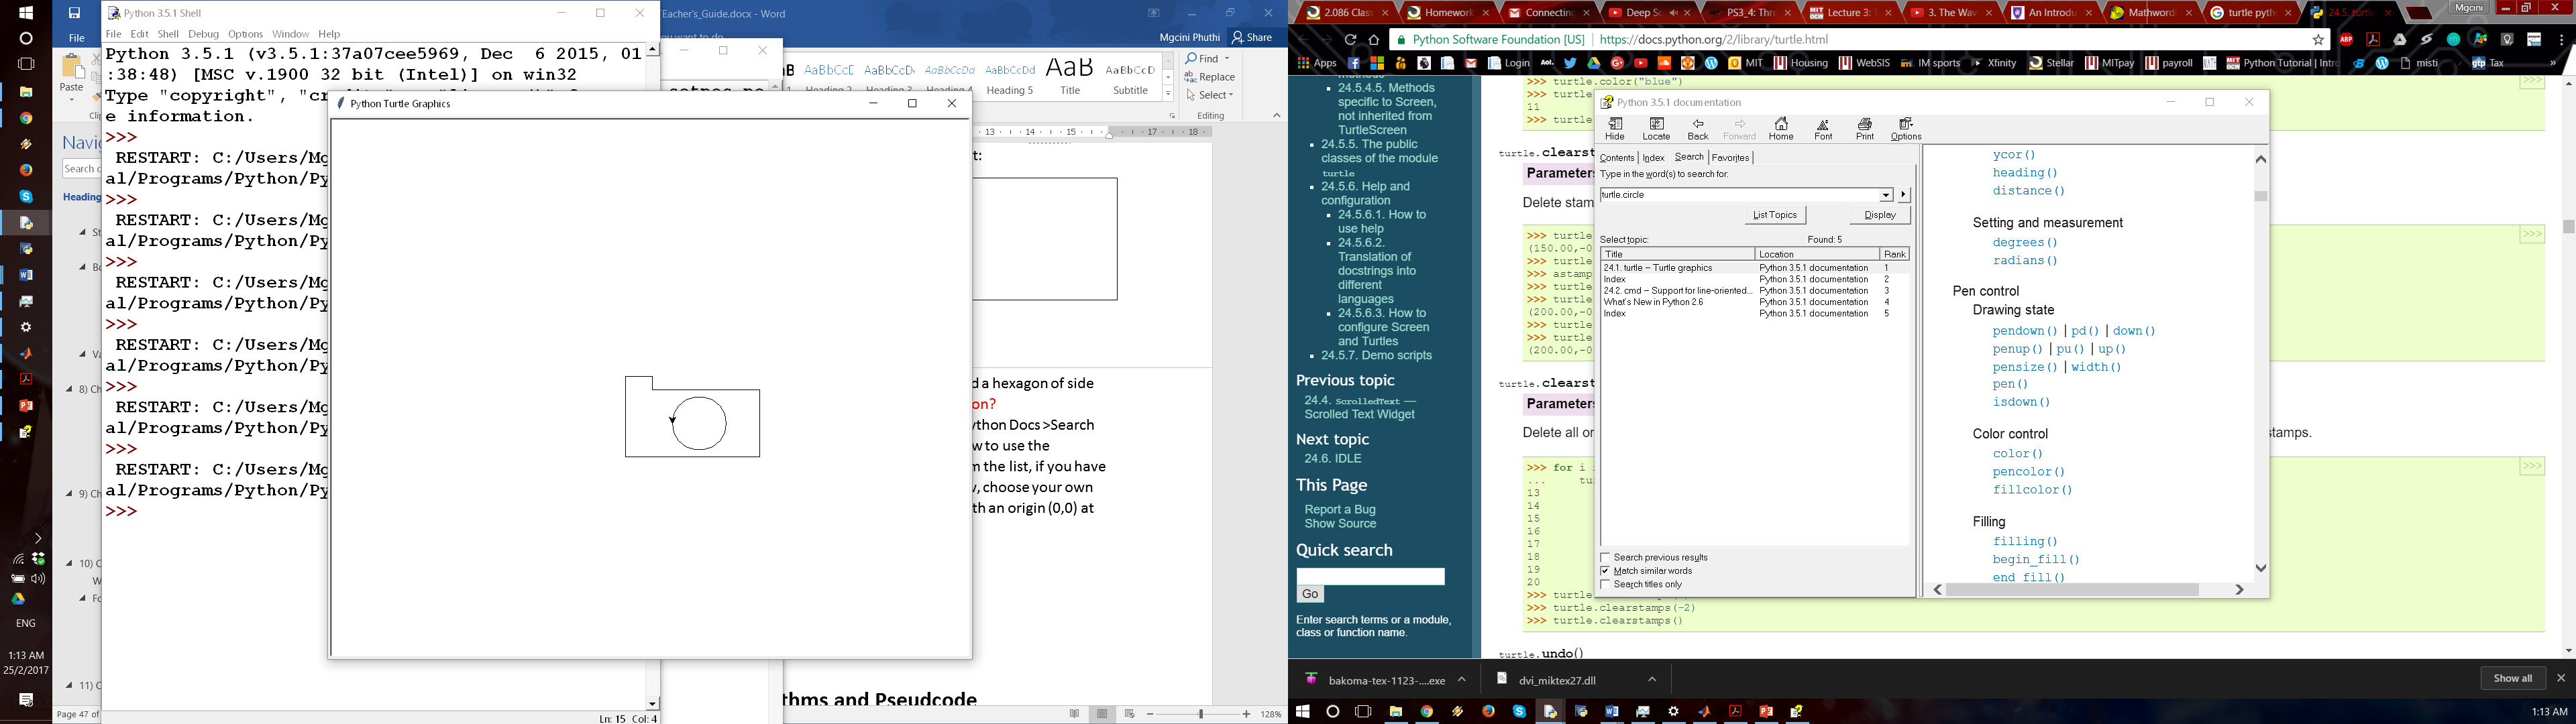
\includegraphics[scale=0.5]{Chapter_One/Figures/b.png}
\caption{What you see when you open IDLE on Windows}
\label{fig:cmd} 
\end{figure}

This is called the Python Shell, it is what allows you to enter in commands one by one. Can you think of another shell we have seen before? 

\subsubsection{Printing to Standard Output}
Now it's time to write our first line of code! In the shell in front of {>}{>}>, type in the following commanc

\begin{shell}
print("Hello World") 
\end{shell}

You have written your first line of code! It tells Python to output/print the words “Hello World” to standard output. Standard output means it just prints the words in the shell after the command is run. Notice how you typed in an input (command), the computer processed that input and it gave you as an output (printed words).

\begin{exercise} \textbf{Say my name}
Change the words inside the quotation marks(") so that it say “Hello” and followed by your name.
Do not remove or add anything else! You have learned your first piece of code using the print()
function!
\end{exercise}

\subsubsection{Arithmetic}
Earlier we said a computer is a calculator, let’s use the computer as a calculator. Execute the
following code, pressing enter after every line to see the output and see if it gives you the right answer. Do not include the things that come after the
“\#” symbol.

\begin{example} Python for calculations
\begin{figure}[h]
\centering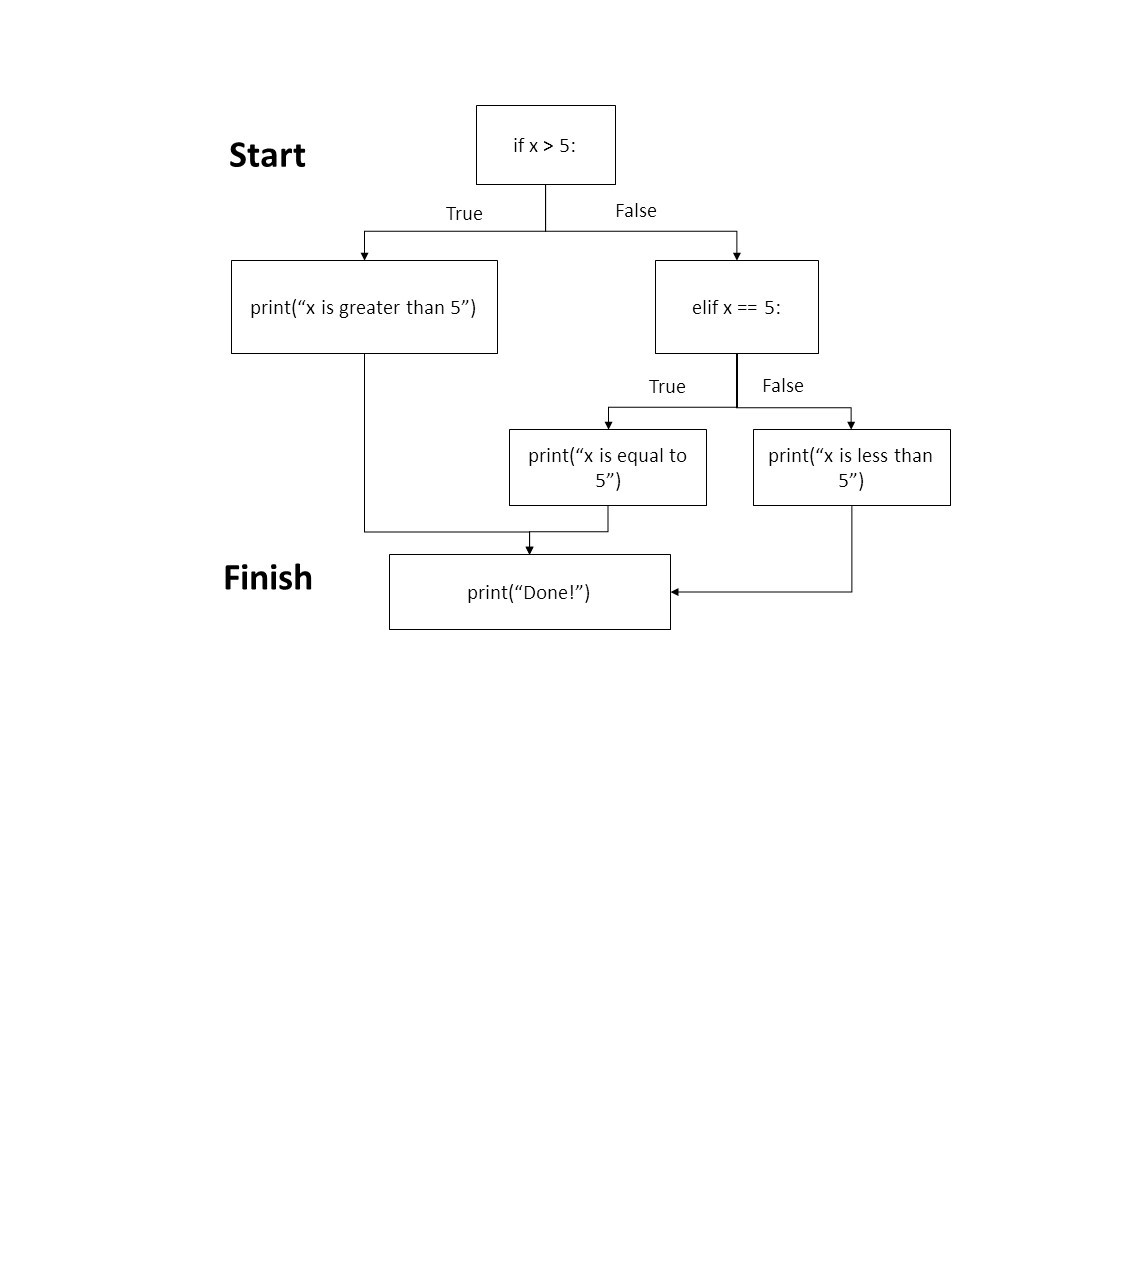
\includegraphics[scale=0.5]{Chapter_One/Figures/c.png}
\caption{Using the Python shell as a calculator}
\label{fig:cmd} 
\end{figure}
\end{example}

\begin{exercise} \textbf{Back to first grade}
Use the symbols you used above to try and do more calculations. Now execute the following code:
\begin{shell}
5//2
3//2
29//5
\end{shell}
\end{exercise}

What do you think the “//” symbol does? This is called floor division, it gives you the whole number from when you divide two numbers. E.g. 5//3 is 1 remainder 2 but the floor division operator only gives you the whole number part which is 1.
Now execute this code and try and figure out what it does.
\begin{shell}
3%2
3%3
3%4
3%7
\end{shell}

The “\%” symbol is called the “mod operator”, it gives you the remainder after division.
Let’s make our calculations a bit more complicated. The rules of BODMAS (Brackets, pOwers,
Division, Multiplication, Addition, Subtraction) that you learned in primary school work here just like for your calculator. Decimals in Python use a full stop which is usually called a period (.), not a
comma (,). Notice that even when you are multiplying things in brackets, you have to put the * operator!

\begin{exercise} BODMAS
Do the following calculation by head and then confirm it on the shell
\begin{shell}

 2*(2)
 2(2) #Why is this an error?
 17//7 + 23%3 + 3**2
 (13+(34/2)*23%4-12)
(23//5)*7/(12%5)+5 \#19.0
((67%5)*(-4*-0.5))**0.5 \#2.0
\end{shell}
\end{exercise}

\subsubsection{Max/Min/Round}
We can also find the maximum and minimum of a group of numbers separated by commas. What 
This is called importing the math module, we will be importing many more modules so remember
how it’s done. 

\begin{shell}
 max(1,2,3,4,5)
 min(1,2,3,4,5)
 max(24,3,7,-3)
 min(23,-4,0,89)
\end{shell}

To round off numbers we use the round() function. 
\begin{shell}
 round(9.4)
 round(9.7)
\end{shell}

\subsubsection{The math module}
If we want to use Python as a scientific calculator, to do this we have to borrow the tools from somewhere else using the following code:
\begin{shell}
 import math
 \end{shell}
 To use the more advanced calculations, we always have to execute the code above. Let’s see what we can do.
\begin{shell}
 math.sqrt(4) #Find squareroot of 4
 math.sin(1) 	#Find sin(1)
 math.pi #The number or pi
 math.cos(math.pi) 	#Find cos(\(\pi\)) or cosine of pi
 math.log10(100) 	#Find log(100) to base 10 
\end{shell}

Remember that this will not work if you do not import the math module first!
\begin{exercise} Scientific calculator
a) Close IDLE and open it again.
b) Calculate the area of a circle of radius 2 using math.pi
c) Copy the answer and round it off to the nearest unit using round()
\end{exercise}

So far you have been typing in commands one by one and executing them, but what if you are
writing some really complicated code like a music player. It would be disaster if it executed your
code right after you’ve typed it, it’s like writing a composition with an examiner who marks after
every sentence. You want to first write out parts of your code, test them and then write more and if you need to change anything, you can go back.
In Python, you can write code using a script which allows you to write a lot of code at once. In IDLE, go to File > New or press Ctrl + N. You should see a blank screen. Type in the “Hello World” code from before and then go to Run > Run Module or press F5. It should give the same output as before.

Now let’s write some more complex code.

\begin{script}
name = input("What is your name?: ")
print("Hi", name) 
\end{script}

This code asks you to type in your name and then when you press enter, it greets you. When you run a script, it never prints anything unless you use the print() function unlike the shell where if you type in a calculation, it immediately gives you an output.

\begin{exercise} \textbf{So many questions}

Change the words inside the quotation marks only so that it asks you different things and gives you a different answer e.g. asking for your age then make it pring “You are 17”. Only edit the text in quotes.
\end{exercise}

\begin{summaryBox} \subsubsection{Summary}
You should now know:
\begin{itemize}
\item That a computer take inputs, processes them and gives outputs, and give examples
\item The basics of what an Operating System and File system are
\item The differences between a GUI and CLI
\item How to make a folder, change directory and open files using both the GUI and CLI
\item That Python is a high level interpreted programming language and what that means
\item What is IDLE and how do you open it?
\item The differences between a script and a shell
\item Writing the Hello World application in both a script and in the python shell
\item How to do basic arithmetic operations as well as using floor, mod operators, min, max and round functions with BODMAS rules
\item How to import import the math module and do basic calculations using cos, sin, pi etc.
\item How to write a simple application that takes input from the user and prints it to standard output
\end{itemize}
\end{summaryBox}
%%------------------------------------------------
%
%\section{Citation}\index{Citation}
%
%This statement requires citation \cite{article_key}; this one is more specific \cite[162]{book_key}.
%
%%------------------------------------------------
%
%\section{Lists}\index{Lists}
%
%Lists are useful to present information in a concise and/or ordered way\footnote{Footnote example...}.
%
%\subsection{Numbered List}\index{Lists!Numbered List}
%
%\begin{enumerate}
%\item The first item
%\item The second item
%\item The third item
%\end{enumerate}
%
%\subsection{Bullet Points}\index{Lists!Bullet Points}
%
%\begin{itemize}
%\item The first item
%\item The second item
%\item The third item
%\end{itemize}
%
%\subsection{Descriptions and Definitions}\index{Lists!Descriptions and Definitions}
%
%\begin{description}
%\item[Name] Description
%\item[Word] Definition
%\item[Comment] Elaboration
%\end{description}
%
%\section{Theorems}\index{Theorems}
%
%This is an example of theorems.
%
%\subsection{Several equations}\index{Theorems!Several Equations}
%This is a theorem consisting of several equations.
%
%\begin{theorem}[Name of the theorem]
%In $E=\mathbb{R}^n$ all norms are equivalent. It has the properties:
%\begin{align}
%& \big| ||\mathbf{x}|| - ||\mathbf{y}|| \big|\leq || \mathbf{x}- \mathbf{y}||\\
%&  ||\sum_{i=1}^n\mathbf{x}_i||\leq \sum_{i=1}^n||\mathbf{x}_i||\quad\text{where $n$ is a finite integer}
%\end{align}
%\end{theorem}
%
%\subsection{Single Line}\index{Theorems!Single Line}
%This is a theorem consisting of just one line.
%
%\begin{theorem}
%A set $\mathcal{D}(G)$ in dense in $L^2(G)$, $|\cdot|_0$. 
%\end{theorem}
%
%%------------------------------------------------
%
%\section{Definitions}\index{Definitions}
%
%This is an example of a definition. A definition could be mathematical or it could define a concept.
%
%\begin{definition}[Definition name]
%Given a vector space $E$, a norm on $E$ is an application, denoted $||\cdot||$, $E$ in $\mathbb{R}^+=[0,+\infty[$ such that:
%\begin{align}
%& ||\mathbf{x}||=0\ \Rightarrow\ \mathbf{x}=\mathbf{0}\\
%& ||\lambda \mathbf{x}||=|\lambda|\cdot ||\mathbf{x}||\\
%& ||\mathbf{x}+\mathbf{y}||\leq ||\mathbf{x}||+||\mathbf{y}||
%\end{align}
%\end{definition}
%
%%------------------------------------------------
%
%\section{Notations}\index{Notations}
%
%\begin{notation}
%Given an open subset $G$ of $\mathbb{R}^n$, the set of functions $\varphi$ are:
%\begin{enumerate}
%\item Bounded support $G$;
%\item Infinitely differentiable;
%\end{enumerate}
%a vector space is denoted by $\mathcal{D}(G)$. 
%\end{notation}
%
%%------------------------------------------------
%
%\section{Remarks}\index{Remarks}
%
%This is an example of a remark.
%
%\begin{remark}
%The concepts presented here are now in conventional employment in mathematics. Vector spaces are taken over the field $\mathbb{K}=\mathbb{R}$, however, established properties are easily extended to $\mathbb{K}=\mathbb{C}$.
%\end{remark}
%
%%------------------------------------------------
%
%\section{Corollaries}\index{Corollaries}
%
%This is an example of a corollary.
%
%\begin{corollary}[Corollary name]
%The concepts presented here are now in conventional employment in mathematics. Vector spaces are taken over the field $\mathbb{K}=\mathbb{R}$, however, established properties are easily extended to $\mathbb{K}=\mathbb{C}$.
%\end{corollary}
%
%%------------------------------------------------
%
%\section{Propositions}\index{Propositions}
%
%This is an example of propositions.
%
%\subsection{Several equations}\index{Propositions!Several Equations}
%
%\begin{proposition}[Proposition name]
%It has the properties:
%\begin{align}
%& \big| ||\mathbf{x}|| - ||\mathbf{y}|| \big|\leq || \mathbf{x}- \mathbf{y}||\\
%&  ||\sum_{i=1}^n\mathbf{x}_i||\leq \sum_{i=1}^n||\mathbf{x}_i||\quad\text{where $n$ is a finite integer}
%\end{align}
%\end{proposition}
%
%\subsection{Single Line}\index{Propositions!Single Line}
%
%\begin{proposition} 
%Let $f,g\in L^2(G)$; if $\forall \varphi\in\mathcal{D}(G)$, $(f,\varphi)_0=(g,\varphi)_0$ then $f = g$. 
%\end{proposition}
%
%%------------------------------------------------
%
%\section{Examples}\index{Examples}
%
%This is an example of examples.
%
%\subsection{Equation and Text}\index{Examples!Equation and Text}
%
%\begin{example}
%Let $G=\{x\in\mathbb{R}^2:|x|<3\}$ and denoted by: $x^0=(1,1)$; consider the function:
%\begin{equation}
%f(x)=\left\{\begin{aligned} & \mathrm{e}^{|x|} & & \text{si $|x-x^0|\leq 1/2$}\\
%& 0 & & \text{si $|x-x^0|> 1/2$}\end{aligned}\right.
%\end{equation}
%The function $f$ has bounded support, we can take $A=\{x\in\mathbb{R}^2:|x-x^0|\leq 1/2+\epsilon\}$ for all $\epsilon\in\intoo{0}{5/2-\sqrt{2}}$.
%\end{example}
%
%\subsection{Paragraph of Text}\index{Examples!Paragraph of Text}
%
%\begin{example}[Example name]
%\lipsum[2]
%\end{example}
%
%%------------------------------------------------
%
%\section{Exercises}\index{Exercises}
%
%This is an example of an exercise.
%
%\begin{exercise}
%This is a good place to ask a question to test learning progress or further cement ideas into students' minds.
%\end{exercise}
%
%%------------------------------------------------
%
%\section{Problems}\index{Problems}
%
%\begin{problem}
%What is the average airspeed velocity of an unladen swallow?
%\end{problem}
%
%%------------------------------------------------
%
%\section{Vocabulary}\index{Vocabulary}
%
%Define a word to improve a students' vocabulary.
%
%\begin{vocabulary}[Word]
%Definition of word.
%\end{vocabulary}
%
%\section{Figure}\index{Figure}
%
%\begin{figure}[h]
%\centering
\includegraphics[scale=0.5]{placeholder.jpg}
%\caption{Figure caption}
%\label{fig:placeholder} % Unique label used for referencing the figure in-text
%%\addcontentsline{toc}{figure}{Figure \ref{fig:placeholder}} % Uncomment to add the figure to the table of contents
%\end{figure}
%
%Referencing Figure \ref{fig:placeholder} in-text automatically.
%
%\section{Table}\index{Table}
%
%\begin{table}[h]
%\centering
%\begin{tabular}{l l l}
%\toprule
%\textbf{Treatments} & \textbf{Response 1} & \textbf{Response 2}\\
%\midrule
%Treatment 1 & 0.0003262 & 0.562 \\
%Treatment 2 & 0.0015681 & 0.910 \\
%Treatment 3 & 0.0009271 & 0.296 \\
%\bottomrule
%\end{tabular}
%\caption{Table caption}
%\label{tab:example} % Unique label used for referencing the table in-text
%%\addcontentsline{toc}{table}{Table \ref{tab:example}} % Uncomment to add the table to the table of contents
%\end{table}
%
%\section{Code}
%
%If code is in a file you can use
%
%\inputminted{python}{Introduction/code.py}
%
%Note that the path must be relative to the main.tex directory\\
%\newline
%For one line code
%
%\mint{html}|<h2>Something <b>here</b></h2>|
%
%For a python script
%
%\begin{script}
%def f():
%	return True
%\end{script}
%
%For a python shell
%
%\begin{shell}
%'1' in '4521'
%\end{shell}
%
%For a cmd prompt
%
%\begin{cmd}
%dir
%cd
%cd ..
%\end{cmd}

\chapterimage{chapter_head_2.pdf} % Chapter heading image

\chapter{Variables}

\section{Abstraction}

So far, we have only been considering things that an ordinary calculator can do with just a few simple
operations. The first and probably the most powerful tool in programming is abstraction. Abstraction
is the use of an idea rather than an event. This is best shown through examples.

\begin{example} \textbf{Using a formula}
If I were to tell you that to calculate the distance travelled by a car I did the following calculation:

\[ distance = 2 * 3 = 6 \]

Is it possible for you to know how I did it? What is 2? What is 3? What units did I use? Is it 6 metres
per second or 6 kilometres per minute? Clearly this is not useful if I want to learn how to calculate
distance by myself. How do we know how to calculate distance? 

The answer is that we know the formula:

\[ distance = speed * time \]

Now, we can calculate any distance given any speed and any time. This is what we mean by
abstraction. Rather than using an event (i.e. exact numbers) we use an idea (i.e. a formula).
\end{example}

\begin{exercise} \textbf{Science – Making a complicated calculation easy}

Imagine that you are the assistant to a crazy physicist named Larmour who needs to know the power
radiated from a point (The point is that this is a complicated calculation, you do not even need to
know what it means). Larmour says he wrote his formula on the board and needs the answer to
finish making a machine that gets rid of all homework so you happily help him. The formula is:
\[ P=\frac{e^2a^2}{6\pi\epsilon_0c^3}\]
He also wrote what number each of the symbols is:

\begin{align*}
e &= 1.6\times 10^{-19} \\
a &= 1\\
\epsilon_0 &= 8.85418782\times 10^{-12}\\
c &= 3\times 10^8\\
\end{align*}

\begin{enumerate}[label=\roman*]
\item What is P? The point is that you can calculate a very complicated thing just because you know the
formula or because Larmour “abstracted” the idea.
\item Suppose Larmour says he made a mistake and a is actually 2, how do you use your answer from i)
to fix this easily?
\end{enumerate}
\end{exercise}

\section{Variables}
Let’s go back to the example with distance where we have:

$$ distance = speed * time $$

We have multiplied before so we know what the “*” does. There are two new things i.e. the three words and the “=” sign. The three words are called variables, which has the same meaning as in mathematics. Variables are containers that hold something e.g. “time” holds the number for a time, “speed” the number for a speed. When we want to calculate the final answer we replace each of those "variables" with the actual number. When calculating the distance and we want an actual number for the distance, we need to know the speed and time first. If we know the speed and time first, we first multiply the numbers on the right and then the “=” sign puts them in the “distance” variable. How do we know it is a variable? Most of the things we are going to work with in Python are going to be variables, except the few cases we will point out.

\begin{exercise} \textbf{Exercise 2.1 – Declaring variables}
In the shell, execute (type it then press enter) the following code:
\begin{shell}
 x = 3
 print(x)
 y = 4
 print(y)
 print(x+y)
 x = y
 print(y)
 name = "Python"      #You can put your own name here
 print(name)
\end{shell}
	
Notice how the letter \icd{x} now stands for 3 and \icd{y} stands for 4 and you can do the things you can do to numbers to x and y because x and y actually represent the numbers in the calculation.
\end{exercise}

\begin{example}\label{example:hands} \textbf{Look, no hands!}
Here is another way to understand variables in Python. Let us say each of your hands is a variable. Your hands can only hold one thing at a time and you have 5 pens of different colors in front of you. Pretend you are a computer, meaning you follow instructions exactly without thinking about it and explain what happens in the following cases (The answers are as simple as you think!)
\begin{enumerate}[label=\alph*]
\item I put (assign) a black pen in your right hand and ask you to write your name.\\
\item I put a red pen in your left hand and ask you to write the date\\
\item If your hands are empty what goes wrong if I ask you to write the time?\\
\item Now let's say you have 3 hands (left, middle and right). What if you have you have a black pen in your right hand, a red pen in your left hand and I ask you to put the black pen in the left hand and red pen in your right hand? You can use your middle hand but you can only have one pen in a hand at a time.
\end{enumerate}
\end{example}

\begin{exercise} \textbf{Python Siri}
\begin{enumerate}[label=\alph*]
\item Now that we can code, we want to make our own  simple version of iPhone’s Siri that can greet someone by their name. Write a script that asks
for the user’s name using \textbf{input()} and then asks for the age and then prints out a greeting that says “Hi, [name], you are [age] years old” where [name] is replaced by the person’s name and [age] is replaced by the person’s age. Think about what variables you can use and how you would name them.
\item Write a script that exchanges the values of two variables \icd{x} and \icd{y}. Think about the demonstration you saw/did and how you would do it in the demonstration and do it in code using only three
lines. (Hint: You can use as many variables as you want)
\end{enumerate}
\end{exercise}

\section{Rules for naming variables}

You may have noticed how much freedom we have when naming variables, this allows us to be able to make smart decisions about how we name them. If you have a long script with lots of variables, you want to be able to know what that variable is easily instead of all your variables being x or y. Here are some rules for naming variables, the first 5 rules are not optional, you will get errors if you do them wrong.

\begin{enumerate}
\item Never use python keywords (e.g. \icd{print}, \icd{def}, \icd{import} etc.) Basically, if the word changes colour when you type it, do not use it as a variable.
\item Do not use the name of a module you have imported (e.g. math). If you import something, its name has been taken, you should not use it for a variable.
\item Do not use any punctuation except underscores ({\_}) in your variable names.
\item Do not use spaces in your variables, if you want to have a space, use an underscore ({\_}) e.g. two{\_}words.
\item Your variable name should never start with a number (e.g. \icd{1st{\_}variable}).
\item Give your variables names that anyone can understand (e.g. \icd{name}, \icd{age}, \icd{number{\_}of{\_}cats}).
\item If your variable is going to be changing, use only lower case letters e.g. \icd{cost{\_}of{\_}food}.
\item If your variable is just a value that you input once at the beginning of the document use all upper case letters e.g. \icd{NUM{\_} WHEELS{\_}{ON}{\_}{CAR}}.
\end{enumerate}

\section{Python keywords and Comments}

Python has special words that mean special things, you can always see a keyword by the way it changes colour when you type it in e.g. \icd{if}, \icd{import}, \icd{elif}, \icd{print} etc. These should never be used as variable names.

We say Python is human readable but sometimes our code gets complicated and someone who did not write the code might want to understand what it does. The person who writes the code can write comments to explain what is going on. Comments always start with the pound sign (aka hashtag) symbol (\#). Anything written on the same line in a different colour after the \# is ignored by Python, so you can write anything you want. Usually they are used to explain steps. You are encouraged to
always write your own comments to explain what you are doing, even to yourself. Here is an example where comments are used:

\begin{script}
x = 1         #Declare a variable x as 1
x += 1        #Add 1 to x
print(x)      #Print the new x
\end{script}

\section{Syntax and Semantics}

So you have been typing code and you have probably run into errors already, for now all the errors you have come across are “syntax” errors. Syntax has to do with rules of a language, things like grammar, spelling and punctuation are the syntax of the English language. Similarly in Python, every bit of code that you type must follow the syntax of Python otherwise you will get a syntax error like the one below when you forget to close the round bracket.

\begin{figure}[h]
\centering
\includegraphics[scale=0.5]{placeholder.jpg}
\caption{Missing figure}
\label{fig:placeholder} % Unique label used for referencing the figure in-text
%\addcontentsline{toc}{figure}{Figure \ref{fig:placeholder}} % Uncomment to add the figure to the table of contents
\end{figure}

Another type of error is what is called a semantic error, this is an error where your code runs but it does not do what you want it to, for example if you want to add two numbers but Python subtracts them instead. Another example is when you say or write something in English but it does not mean what you think it means even though it is spelled and punctuated correctly. These errors are very dangerous because Python will not tell you that your code is wrong, so you have to test your code and if it has problems, you “debug” it. Debugging means fixing code that does not work properly.

\begin{toolbox} \textbf{The basics}
\begin{enumerate}
\item Variables
\item Comments
\item Coding vocabulary (syntax, semantics, debugging)
\end{enumerate}
\end{toolbox}


%\chapter{Introduction to Computers and Programming}

%\section{Paragraphs of Text}\index{Paragraphs of Text}
%Blah blah blah
%
%%------------------------------------------------
%
%\section{Citation}\index{Citation}
%
%This statement requires citation \cite{article_key}; this one is more specific \cite[162]{book_key}.
%
%%------------------------------------------------
%
%\section{Lists}\index{Lists}
%
%Lists are useful to present information in a concise and/or ordered way\footnote{Footnote example...}.
%
%\subsection{Numbered List}\index{Lists!Numbered List}
%
%\begin{enumerate}
%\item The first item
%\item The second item
%\item The third item
%\end{enumerate}
%
%\subsection{Bullet Points}\index{Lists!Bullet Points}
%
%\begin{itemize}
%\item The first item
%\item The second item
%\item The third item
%\end{itemize}
%
%\subsection{Descriptions and Definitions}\index{Lists!Descriptions and Definitions}
%
%\begin{description}
%\item[Name] Description
%\item[Word] Definition
%\item[Comment] Elaboration
%\end{description}
%
%\section{Theorems}\index{Theorems}
%
%This is an example of theorems.
%
%\subsection{Several equations}\index{Theorems!Several Equations}
%This is a theorem consisting of several equations.
%
%\begin{theorem}[Name of the theorem]
%In $E=\mathbb{R}^n$ all norms are equivalent. It has the properties:
%\begin{align}
%& \big| ||\mathbf{x}|| - ||\mathbf{y}|| \big|\leq || \mathbf{x}- \mathbf{y}||\\
%&  ||\sum_{i=1}^n\mathbf{x}_i||\leq \sum_{i=1}^n||\mathbf{x}_i||\quad\text{where $n$ is a finite integer}
%\end{align}
%\end{theorem}
%
%\subsection{Single Line}\index{Theorems!Single Line}
%This is a theorem consisting of just one line.
%
%\begin{theorem}
%A set $\mathcal{D}(G)$ in dense in $L^2(G)$, $|\cdot|_0$. 
%\end{theorem}
%
%%------------------------------------------------
%
%\section{Definitions}\index{Definitions}
%
%This is an example of a definition. A definition could be mathematical or it could define a concept.
%
%\begin{definition}[Definition name]
%Given a vector space $E$, a norm on $E$ is an application, denoted $||\cdot||$, $E$ in $\mathbb{R}^+=[0,+\infty[$ such that:
%\begin{align}
%& ||\mathbf{x}||=0\ \Rightarrow\ \mathbf{x}=\mathbf{0}\\
%& ||\lambda \mathbf{x}||=|\lambda|\cdot ||\mathbf{x}||\\
%& ||\mathbf{x}+\mathbf{y}||\leq ||\mathbf{x}||+||\mathbf{y}||
%\end{align}
%\end{definition}
%
%%------------------------------------------------
%
%\section{Notations}\index{Notations}
%
%\begin{notation}
%Given an open subset $G$ of $\mathbb{R}^n$, the set of functions $\varphi$ are:
%\begin{enumerate}
%\item Bounded support $G$;
%\item Infinitely differentiable;
%\end{enumerate}
%a vector space is denoted by $\mathcal{D}(G)$. 
%\end{notation}
%
%%------------------------------------------------
%
%\section{Remarks}\index{Remarks}
%
%This is an example of a remark.
%
%\begin{remark}
%The concepts presented here are now in conventional employment in mathematics. Vector spaces are taken over the field $\mathbb{K}=\mathbb{R}$, however, established properties are easily extended to $\mathbb{K}=\mathbb{C}$.
%\end{remark}
%
%%------------------------------------------------
%
%\section{Corollaries}\index{Corollaries}
%
%This is an example of a corollary.
%
%\begin{corollary}[Corollary name]
%The concepts presented here are now in conventional employment in mathematics. Vector spaces are taken over the field $\mathbb{K}=\mathbb{R}$, however, established properties are easily extended to $\mathbb{K}=\mathbb{C}$.
%\end{corollary}
%
%%------------------------------------------------
%
%\section{Propositions}\index{Propositions}
%
%This is an example of propositions.
%
%\subsection{Several equations}\index{Propositions!Several Equations}
%
%\begin{proposition}[Proposition name]
%It has the properties:
%\begin{align}
%& \big| ||\mathbf{x}|| - ||\mathbf{y}|| \big|\leq || \mathbf{x}- \mathbf{y}||\\
%&  ||\sum_{i=1}^n\mathbf{x}_i||\leq \sum_{i=1}^n||\mathbf{x}_i||\quad\text{where $n$ is a finite integer}
%\end{align}
%\end{proposition}
%
%\subsection{Single Line}\index{Propositions!Single Line}
%
%\begin{proposition} 
%Let $f,g\in L^2(G)$; if $\forall \varphi\in\mathcal{D}(G)$, $(f,\varphi)_0=(g,\varphi)_0$ then $f = g$. 
%\end{proposition}
%
%%------------------------------------------------
%
%\section{Examples}\index{Examples}
%
%This is an example of examples.
%
%\subsection{Equation and Text}\index{Examples!Equation and Text}
%
%\begin{example}
%Let $G=\{x\in\mathbb{R}^2:|x|<3\}$ and denoted by: $x^0=(1,1)$; consider the function:
%\begin{equation}
%f(x)=\left\{\begin{aligned} & \mathrm{e}^{|x|} & & \text{si $|x-x^0|\leq 1/2$}\\
%& 0 & & \text{si $|x-x^0|> 1/2$}\end{aligned}\right.
%\end{equation}
%The function $f$ has bounded support, we can take $A=\{x\in\mathbb{R}^2:|x-x^0|\leq 1/2+\epsilon\}$ for all $\epsilon\in\intoo{0}{5/2-\sqrt{2}}$.
%\end{example}
%
%\subsection{Paragraph of Text}\index{Examples!Paragraph of Text}
%
%\begin{example}[Example name]
%\lipsum[2]
%\end{example}
%
%%------------------------------------------------
%
%\section{Exercises}\index{Exercises}
%
%This is an example of an exercise.
%
%\begin{exercise}
%This is a good place to ask a question to test learning progress or further cement ideas into students' minds.
%\end{exercise}
%
%%------------------------------------------------
%
%\section{Problems}\index{Problems}
%
%\begin{problem}
%What is the average airspeed velocity of an unladen swallow?
%\end{problem}
%
%%------------------------------------------------
%
%\section{Vocabulary}\index{Vocabulary}
%
%Define a word to improve a students' vocabulary.
%%
%%\begin{vocabulary}[Word]
%%Definition of word.
%%\end{vocabulary}
%%
%%\section{Figure}\index{Figure}
%%
%%\begin{figure}[h]
%%\centering
\includegraphics[scale=0.5]{placeholder.jpg}
%%\caption{Figure caption}
%%\label{fig:placeholder} % Unique label used for referencing the figure in-text
%%\addcontentsline{toc}{figure}{Figure \ref{fig:placeholder}} % Uncomment to add the figure to the table of contents
%%\end{figure}
%
%Referencing Figure \ref{fig:placeholder} in-text automatically.
%
%\section{Table}\index{Table}
%
%\begin{table}[h]
%\centering
%\begin{tabular}{l l l}
%\toprule
%\textbf{Treatments} & \textbf{Response 1} & \textbf{Response 2}\\
%\midrule
%Treatment 1 & 0.0003262 & 0.562 \\
%Treatment 2 & 0.0015681 & 0.910 \\
%Treatment 3 & 0.0009271 & 0.296 \\
%\bottomrule
%\end{tabular}
%\caption{Table caption}
%\label{tab:example} % Unique label used for referencing the table in-text
%\addcontentsline{toc}{table}{Table \ref{tab:example}} % Uncomment to add the table to the table of contents
%\end{table}
%
%\section{Code}
%
%If code is in a file you can use
%
%%\inputminted{python}{Introduction/code.py}
%
%Note that the path must be relative to the main.tex directory\\
%\newline
%For one line code
%
%\mint{html}|<h2>Something <b>here</b></h2>|
%
%For a python script
%
%\begin{script}
%def f():
%	return True
%\end{script}
%
%For a python shell
%
%\begin{shell}
%'1' in '4521'
%\end{shell}
%
%For a cmd prompt
%
%\begin{cmd}
%dir
%cd
%cd ..
%\end{cmd}

%\include{Chapter_Three/Chapter_Three}


%----------------------------------------------------------------------------------------
%	PART
%----------------------------------------------------------------------------------------

\part{Part Two}

%----------------------------------------------------------------------------------------
%	CHAPTER 3
%----------------------------------------------------------------------------------------

\chapterimage{chapter_head_1.pdf} % Chapter heading image

\chapter{Presenting Information}

Referencing Table \ref{tab:example} in-text automatically.

%------------------------------------------------


%----------------------------------------------------------------------------------------
%	BIBLIOGRAPHY
%----------------------------------------------------------------------------------------

\chapter*{Bibliography}
\addcontentsline{toc}{chapter}{\textcolor{ocre}{Bibliography}} % Add a Bibliography heading to the table of contents

%------------------------------------------------

\section*{Articles}
\addcontentsline{toc}{section}{Articles}
\printbibliography[heading=bibempty,type=article]

%------------------------------------------------

\section*{Books}
\addcontentsline{toc}{section}{Books}
\printbibliography[heading=bibempty,type=book]

%----------------------------------------------------------------------------------------
%	INDEX
%----------------------------------------------------------------------------------------

\cleardoublepage % Make sure the index starts on an odd (right side) page
\phantomsection
\setlength{\columnsep}{0.75cm} % Space between the 2 columns of the index
\addcontentsline{toc}{chapter}{\textcolor{ocre}{Index}} % Add an Index heading to the table of contents
\printindex % Output the index

%----------------------------------------------------------------------------------------

\end{document}
